\section{Experiments}
\label{sec:experiments}

We evaluate four distinct questions: local autonomous prediction,
cross-regime assembly, routing behavior and physical consistency,
and computational cost. The benchmarks have complementary roles,
not an identical matrix of experiments. Fluidic pinball provides an
archived comparison with POD--Galerkin; the circular cylinder provides
controlled local-model comparisons; and the centered square provides
the principal fusion ablations. Benchmark configurations are given in
Table~\ref{tab:chart_splits}.

\paragraph{Evaluation scope.}
We denote the joint physical-field error by $E_{\mathrm{joint}}=E_u+E_p$.
The Circular controls and Square fusion study use full-window errors
against POD-reconstructed reference fields, excluding the raw-field
projection remainder. Square terminal-step errors are supplementary
and are not mixed with full-window averages. Neural local-model seeds,
gate-only seeds, and frozen-model diagnostics are reported separately.
The experimental appendices follow the same four-part order and provide
protocols, component results, and supplementary diagnostics.



\subsection{Local prediction accuracy and finite-horizon reliability}
\label{sec:exp_local}

\paragraph{Pinball: archived prediction versus POD--Galerkin.}
Table~\ref{tab:pinball_autonomous} compares archived learned local
predictors with POD--Galerkin over $K=32$--$56$ steps. In the three
settings with a recorded baseline, the learned predictor has lower
velocity and pressure errors. The Steady baseline is unavailable.
The Periodic learned predictor is identified as Deep-FNN-H3; the
architecture of the earlier standalone Steady/Hopf rows is not fully
resolved. We therefore retain this comparison as evidence about the
archived predictors, not as an ablation attributing improvement to
sparse MoE. Appendix~\ref{app:pinball} specifies the provenance and
Periodic-core cadence. These finite-horizon results do not establish
arbitrary-time stability.


\begin{table}[H]
\centering
\caption{
Archived autonomous prediction on fluidic pinball. Errors are
physical-field percentages. ``Archived learned'' does not assert a
verified sparse-MoE architecture; the Periodic rows are Deep-FNN-H3.
Dashes denote an unavailable baseline, not divergence.
Periodic-core uses the longer evaluation in Appendix~\ref{app:pinball}.
}
\label{tab:pinball_autonomous}
\small
\setlength{\tabcolsep}{5pt}
\begin{tabular}{@{}llrrr@{}}
\toprule
Evaluation setting & Model & $E_u$ & $E_p$ & $E_{\mathrm{joint}}$ \\
\midrule
Steady ($K=56$)
& POD--Galerkin
& -- & -- & -- \\
& Archived learned
& 0.2247 & 0.7593 & 0.9840 \\
\addlinespace

Hopf ($K=56$)
& POD--Galerkin
& 0.4378 & 48.50 & 48.94 \\
& Archived learned
& 0.0995 & 1.986 & 2.085 \\
\addlinespace

Periodic ($K=32$)
& POD--Galerkin
& 1.641 & 41.56 & 43.20 \\
& Deep-FNN-H3
& 0.2897 & 0.5518 & 0.8415 \\
\addlinespace

Periodic-core ($K=56$)
& POD--Galerkin
& 2.555 & 39.36 & 41.91 \\
& Deep-FNN-H3
& 0.6222 & 1.050 & 1.672 \\
\bottomrule
\end{tabular}
\end{table}

\paragraph{Circular: controlled local architecture comparisons.}
We compare Circular Hopf and Periodic predictors on common held-out
windows at $K=24$ and $K=48$, using seeds 1248, 1600, and 2026 for
the neural configurations. This is a separate study from the Pinball
baseline comparison: it tests architecture and training sensitivity.
Dense matches the proposed model's active
neural parameter budget, while Structured retains explicit response
branches but removes input-dependent expert routing. These are
controls for the local architecture, not substitutes for a bare
POD--Galerkin ablation. We also include a validation-selected
operator inference (OpInf) fit as an external ROM comparison.
The repaired configurations change the initialization of the
low-rank quadratic factors; they are retrained models, not a
post-hoc modification of the original predictions.

Table~\ref{tab:circular_full_reorg} brings together both regimes and
horizons under the same full-window joint-error metric.
Reference fields are reconstructed from true POD coefficients, so
these errors exclude the original CFD projection remainder.
Evaluation windows, aggregation, component errors, and implementation
details are provided in Appendix~\ref{app:circular}.

\begin{table}[H]
\centering
\small
\setlength{\tabcolsep}{4pt}
\caption{Circular local controls: full-window joint error
$E_u+E_p$ (\%) against POD-reconstructed reference fields.
Neural entries are mean $\pm$ sample standard deviation over accepted
seeds among three attempts. Accepted seed sets can differ between
configurations; 2/3 rows are conditional descriptive statistics,
not complete three-seed estimates. Repaired Hopf rows use FP32.
OpInf is a single deterministic validation-selected fit.
The two horizons use the same windows, with $K=24$ restricted to
their first 24 steps.}
\label{tab:circular_full_reorg}
\begin{tabular}{@{}llccc@{}}
\toprule
Regime & Model & $K=24$ & $K=48$ & Accepted\\
\midrule
Hopf & Proposed, original
& $0.11521\pm0.08694$ & $0.11487\pm0.10033$ & 2/3\\
& Proposed, repaired
& $0.04334\pm0.02379$ & $0.05044\pm0.03439$ & 2/3\\
& Dense, active-matched
& $0.15406\pm0.16364$ & $0.15480\pm0.15525$ & 2/3\\
& Structured, original
& $0.12537\pm0.04614$ & $0.12724\pm0.04302$ & 3/3\\
& Structured, repaired
& $0.02229\pm0.00432$ & $0.02392\pm0.00778$ & 2/3\\
& OpInf & 0.03870 & 0.05340 & Deterministic\\
\midrule
Periodic & Proposed, original
& $2.8791\pm1.7269$ & $4.9443\pm3.1576$ & 3/3\\
& Proposed, repaired
& $3.0667\pm1.8373$ & $5.5322\pm3.6623$ & 3/3\\
& Dense, active-matched
& $\mathbf{1.3251\pm0.2268}$ & $\mathbf{2.3998\pm0.6599}$ & 3/3\\
& Structured, original
& $2.8666\pm1.4342$ & $5.2810\pm2.5679$ & 3/3\\
& Structured, repaired
& $2.8598\pm1.3081$ & $5.0677\pm2.3762$ & 3/3\\
& OpInf & 114.0941 & 114.9897 & Deterministic\\
\bottomrule
\end{tabular}
\end{table}

\paragraph{Architecture and external-baseline results.}
All Periodic neural configurations have three accepted seeds.
Dense yields lower mean joint errors than the proposed configurations
at both horizons, while Structured is close to the original proposed
model. Under this active-parameter budget and evaluation protocol,
the results therefore do not establish a Periodic accuracy advantage
from input-dependent sparse routing. Errors increase when extending
the window from 24 to 48 steps; neither low finite-window error nor
successful completion proves arbitrary-time stability.
The validation-selected OpInf fit is competitive on Hopf but much
less accurate on Periodic. Its Periodic ridge parameter reaches the
search-grid upper boundary; its pressure parameterization and derivative
estimation also differ from the neural models
(Appendix~\ref{app:circular}). This task-specific comparison does not
establish superiority over the OpInf method family.

\paragraph{Initialization and training reliability.}
The original Circular quadratic branches remain inactive because
both multiplicative factors were initialized at zero.
Retaining one random factor while zeroing the other permits learning,
but the repaired Proposed model does not improve the Periodic mean
error. Retraining also changes optimization and checkpoint selection,
so this comparison does not isolate the quadratic term alone.
For Hopf, repaired FP32 configurations have only two accepted seeds
per architecture, and their accepted sets differ from the original
ones. Their lower conditional errors consequently do not establish
improved expected performance or complete three-seed robustness.
Appendix~\ref{app:circular} reports the initialization mechanism and
Table~\ref{tab:hopf_completion} distinguishes training failure from
validation rejection.

\subsection{Cross-regime routing and physical-space fusion}
\label{sec:exp_fusion}

\paragraph{Square: selection and fusion controls.}
We hold the Square local predictors and E2 router fixed and compare
assembly rules on the prescribed S--H and H--P support at $K=24$.
Each interface contains 16 held-out windows.
E2 Top-1 selects within the supplied pair; T2-C learns a correction
to its pair preference using initial-history descriptors.
Neither the candidate set nor an automatic applicability mask is
learned in this experiment.

Table~\ref{tab:routing_fusion} uses a common full-window metric.
Train-fixed $\alpha$ and train-fixed logit offset are fitted only
on training windows, and the fixed candidate is selected on
validation error. These controls test whether the improvement
can be explained by a constant mixture or calibration offset.

\begin{table}[H]
\centering
\small
\caption{Square full-window joint error (\%) at $K=24$ against the
cached POD reference. Entries use the frozen-checkpoint reevaluation,
not a three-seed average. Scalar controls use training data;
the fixed candidate uses validation data.}
\label{tab:routing_fusion}
\begin{tabular}{@{}lrr@{}}
\toprule
Assembly rule & S--H & H--P\\
\midrule
E2 Top-1 & 1.5786 & 1.6424\\
E2-probability blend & 1.8145 & 1.4489\\
Equal blend & 2.3849 & 1.3930\\
Train-fixed $\alpha$ & 2.0591 & 0.9767\\
Train-fixed logit offset & 2.0149 & 0.9821\\
Validation-fixed candidate & 1.5786 & 1.0068\\
T2-C & \textbf{1.0954} & \textbf{0.8123}\\
\bottomrule
\end{tabular}
\end{table}

\paragraph{Square: history conditioning and gate variability.}
T2-C improves on all listed controls for these fixed candidate
sets. A separate architecture-matched $\mu$-only control zeros the
standardized history channels while retaining the gate architecture.
Across three paired gate seeds, full-window joint errors are
$1.095351\pm0.000015\%$ versus $1.814699\pm0.000242\%$
in S--H and $0.812343\pm0.000177\%$ versus
$0.976939\pm0.000179\%$ in H--P.
The reductions are $39.64\%$ and $16.85\%$.
These quantify gate-training variability, not uncertainty from
retraining the complete hierarchy.

\begin{figure}[H]
\centering
% Source: audited three-gate-seed full-window means; no field pixels generated.
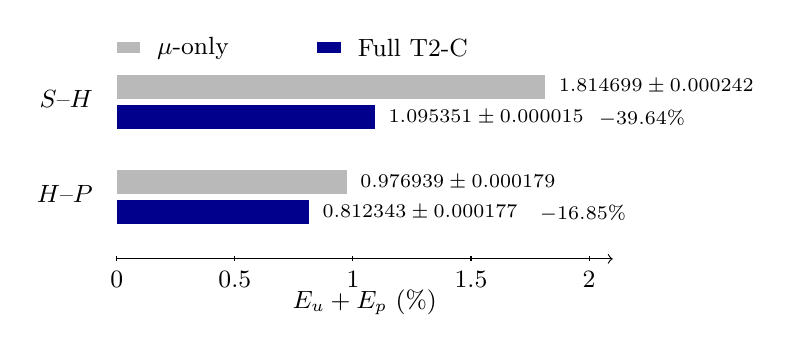
\begin{tikzpicture}[x=3cm,y=0.55cm,font=\small]
\draw[->] (0,0)--(2.1,0);
\node at (1.05,-1.0) {$E_u+E_p$ (\%)};
\foreach \t in {0,0.5,1,1.5,2} {
 \draw (\t,0.06)--(\t,-0.06) node[below] {\t};
}
\node[anchor=east] at (-0.06,3.7) {$S$--$H$};
\node[anchor=east] at (-0.06,1.5) {$H$--$P$};
\fill[gray!55] (0,3.7) rectangle (1.814699,4.25);
\fill[blue!55!black] (0,3.0) rectangle (1.095351,3.55);
\fill[gray!55] (0,1.5) rectangle (0.976939,2.05);
\fill[blue!55!black] (0,0.8) rectangle (0.812343,1.35);
\node[anchor=west,font=\scriptsize] at (1.83,3.975) {$1.814699\pm0.000242$};
\node[anchor=west,font=\scriptsize] at (1.11,3.275) {$1.095351\pm0.000015$};
\node[anchor=west,font=\scriptsize] at (0.99,1.775) {$0.976939\pm0.000179$};
\node[anchor=west,font=\scriptsize] at (0.83,1.075) {$0.812343\pm0.000177$};
\fill[gray!55] (0,4.75) rectangle (0.1,5.0);
\node[anchor=west] at (0.13,4.87) {$\mu$-only};
\fill[blue!55!black] (0.85,4.75) rectangle (0.95,5.0);
\node[anchor=west] at (0.98,4.87) {Full T2-C};
\node[anchor=west,font=\scriptsize] at (2.0,3.25) {$-39.64\%$};
\node[anchor=west,font=\scriptsize] at (1.75,1.05) {$-16.85\%$};
\end{tikzpicture}

\caption{Full-window Square comparison over three paired gate seeds.
All local candidates and E2 are fixed; bars show mean and sample
standard deviation.}
\label{fig:square_overlap}
\end{figure}

The evidence supports history-conditioned fusion for these windows,
but does not prove that history dependence is necessary for every
flow or gate. The weight is fixed within each prediction window;
history can change it between windows.
Appendices~\ref{app:square}--\ref{app:square_terminal} retain component errors, terminal-step
results, scalar objectives, and complete field visualizations.
A posteriori convex oracles are diagnostics, not deployable methods.

\paragraph{Pinball: supplementary transfer of the assembly rule.}
Appendix~\ref{app:pinball_overlap_results} reports S--H and H--P
overlap results at $K=24,56$. T2-C improves on the better individual
candidate in all four archived settings. The local candidates are
Deep-FNN-H3, so these results test physical-space assembly rather than
the sparse-MoE architecture. They do not replicate the full Square
scalar-control and gate-seed study.

\subsection{Internal routing and physical-field diagnostics}
\label{sec:exp_diagnostics}

\paragraph{Circular: internal expert utilization.}
Post-hoc diagnostics use frozen original Circular H/P specialists,
not the repaired three-seed models, and are not used for checkpoint
selection. The H study uses 15 windows at $K=56$ and the P study
52 windows at $K=48$; these differ from the 42 H and 32 P windows
of the controlled local comparison.
Periodic distributes decisions across group--pair combinations;
Hopf has a prescribed single group and fixed sparse support, but
nonuniform, parameter-dependent mixture weights.
Its single group is not evidence of collapse of a learned
multi-group router. The detailed frequency, weight-mass, and entropy
statistics in Appendix~\ref{app:internal_routing} count the first
integration stage per output step, not all RK evaluations.
Utilization alone does not establish an accuracy benefit.

\paragraph{Square: measured fusion consistency.}
Appendix~\ref{app:fusion_consistency} gives conditional algebraic
identities; Appendix~\ref{app:fusion_measured} reports the separate
reconstructed-field measurements. The measured
study uses the same 16 windows per interface and $K=24$ as the Square
fusion evaluation, comparing each candidate, the frozen T2-C blend,
and the common POD reference.
On both Square interfaces, the measured T2-C pressure residual is
lower than either candidate for both tested spatial stencils.
However, Hopf has a smaller H--P momentum residual and a smaller
S--H energy error. Fusion is therefore not a general residual or
energy-error minimizer.

The measurements use offline least-squares spatial derivatives
and coarse-time differences, not the original OpenFOAM
finite-volume residuals. Nonzero reference residuals include POD
truncation and differentiation error.
Identity discrepancies near machine precision verify the algebra,
not conservation or physical accuracy.
The phase screen resolves none of the 16 S--H windows and 15 of
16 H--P windows; even resolved short-window traces do not establish
absence of aliasing or long-time phase stability.
The complete energy, residual, probe, and phase curves are retained
in Appendix~\ref{app:fusion_measured}.

\subsection{Computational cost and timing boundaries}
\label{sec:exp_cost}

\paragraph{Circular: parameter use and local latency.}
Sparse activation is a parameter-use property, not a runtime claim.
Circular H/P activate $44.53\%$ and $17.09\%$ of their trainable
parameters per analyzed prediction decision.
For native Circular Periodic prediction at batch size one and
$K=48$, median times are 2.1848 s (proposed), 0.6579 s (Dense),
and 0.8652 s (Structured).
The proposed implementation is therefore slower than Dense in this
measurement despite sparse activation; the native Galerkin path
also executes on the CPU.

\paragraph{Circular Periodic: a physical-window-matched FOM reference.}
A separate warm physical-input/physical-output measurement includes
history encoding, local advancement, and all-step field decoding.
It takes 2.18747 s on an RTX 4090 with a Xeon host for a Circular
Periodic window spanning 598.70093 physical time units.
A matched historical production FOM interval takes 1996 s.
The resulting ratio of approximately 912.5 is not a full-hierarchy
or hardware-independent speedup: hardware and I/O boundaries differ,
the FOM timing has one realization, and ROM loading, output writes,
E2, descriptors, and T2-C are excluded.
Appendix~\ref{app:parameter_counts} lists warm-ups, repetitions,
synchronization, memory, hardware, and all included/excluded work.
A fully paired Top-2 end-to-end timing remains unmeasured.
